\section{Technical facts}
\subsection{Polynomial time balanced sparse cut algorithm}
\label{apndx:selfloops}
In this section, we prove the following fast BSCA, used for our polynomial time BLD construction.

\fastbalsparse*

\begin{proof}
	First we show how to reduce the BSCA task on graphs with self-loops to graphs without self-loops. Let $G=(V,E,w)$ be a weighted undirected graph with one weighted self-loop per vertex, where $w: E \cup V \rightarrow \mathbb{R}_{\ge 0}$ and $E \subseteq \binom{V}{2}$. The idea is to construct a graph with two copies of every vertex, where the surplus vertices are solely connected to their corresponding vertex with weight equal to half the weight of the self-loop. If a vertex has no self-loops then we make only one copy for it. Formally, let $A=\{u \in V:w(u) > 0\}$ be the set of vertices with self-loops. Then let $B$ be a copy of $A$ representing the self-loops of vertices in $A$, and let $s: A \rightarrow B$ be a bijection mapping $u \in A$ to its corresponding self-loop vertex $s(u) \in B$. We define the self-loop free graph to be $\hat{G}=(\hat{V},\hat{E},\hat{w})$, where $\hat{V} = V \cup s(A)$, $\hat{E}=E \cup (\cup_{u \in A} \{\{u, s(u)\}\})$, and $\hat{w}(e)=w(e)$ for every $e \in E$ and $\hat{w}(\{u, s(u)\})=\frac{1}{2}w(u)$ for all $u \in A$. This is illustrated in \Cref{fig:selfloopsredcution}. We highlight that $\hat{G}$ has the same number of vertices and edges as $G$, up to constants.

\begin{figure}[h]
	\begin{minipage}[center]{\textwidth}
		\centering
		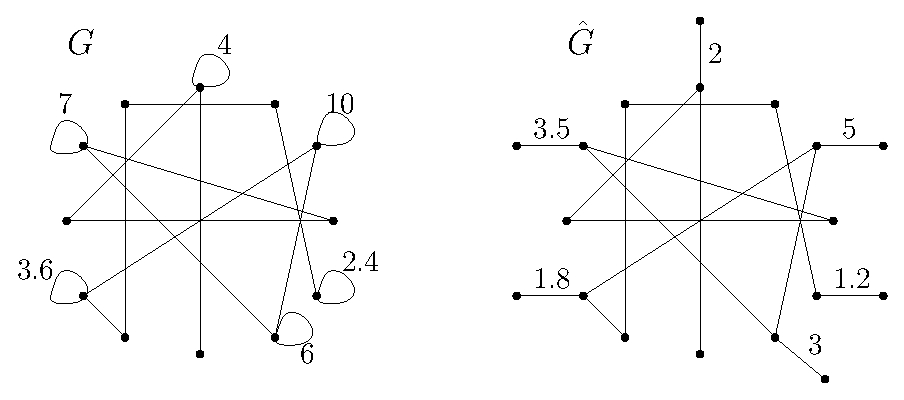
\includegraphics[scale=0.9]{selfloops_reduction.eps}
	\end{minipage}
	\caption{On the left: the original graph with self-loops $G$. On the right: its self-loop free version~$\hat{G}$. The weights of the internal edges of $G$ are copied verbatim (not shown in the figure), while the weights of self-loops are halved.}
	\label{fig:selfloopsredcution}
\end{figure}

\noindent
We run a BSCA for self-loop free graphs on $\hat{G}$, and if it asserts $\hat{G}$ to be an expander we conclude the same for $G$, whereas if it returns a cut then we tweak it to get a solution for $G$. This is summarised in Algorithm~\ref{alg:selfloop}. The following claim gives the correctness of the reduction. The idea is that the subgraphs given by $\{u,s(u)\}$ for $u \in A$ are expanders, so there is no good reason for a sparse cut to cross them. Hence, $u$ and $s(u)$ should be on the same side of the sparse cuts.


\begin{algorithm}[h]
	\caption{\textsc{SelfLoopBalSparseCut}: reduction to self-loop free BSCA}
	\label{alg:selfloop}
	\begin{algorithmic}[1]
		\LeftComment{$G=(V,E,w)$ is a weighted undirected graph}
		\LeftComment{$\phi \in (0,1)$ is the sparsity parameter}
		\Procedure{\textsc{SelfLoopBalSparseCut}$(G,\phi)$}{}
		\State $\hat{\omega} \gets \bsc(\hat{G},\phi)$ \Comment{$\hat{G}$ is the self-loop free version of $G$ as described above}
		\If{$\hat{\omega} = \bot$}
			\State $\omega \gets \bot$
		\Else
		\State $(R,\nu) \gets \hat{\omega}$
		\State $X \gets R \cap V$
		\State $X^* \gets \argmin\{\vol_G(X),\vol_G(V \setminus X)\}$
		\State $\omega \gets (X^*, \vol_G(X^*))$
		\EndIf
		\State \Return $\omega$
		\EndProcedure
	\end{algorithmic}
\end{algorithm}

\begin{claim}
	\label{lem:selfloopfree}
	Let $\bsc$ be an $(\alpha,\lambda)$-BSCA. Then \textsc{SelfLoopBalSparseCut} is a $(2\alpha,4\lambda)$-BSCA, provided that the input sparsity parameter $\phi \in (0,1)$ satisfies $\phi \le \frac{1}{10\alpha}$.
\end{claim}
\begin{proof}
	For any cut $\emptyset \neq X \subsetneq V$, let us define for convenience $\partial_G X=w(X,V \setminus X)$ to be the total weight of the edges crossing the cut $X$ in $G$, and for any cut \smash{$\emptyset \neq R \subsetneq \hat{V}$} define \smash{$\partial_{\hat{G}} R=\hat{w}(R,\hat{V}\setminus R)$} to be the total weight of edges crossing $R$ in $\hat{G}$. A preliminary observation is that for any cut $\emptyset \neq X \subsetneq V$ we have that \smash{$\vol_{\hat{G}}(X \cup s(X \cap A))=\vol_G(X)$}, \smash{$\partial_{\hat{G}} (X \cup s(X \cap A)) = \partial_G X$}, and consequently \smash{$\Phi_{\hat{G}}(X \cup s(X \cap A)) = \Phi_G(X)$}. By definition of $\bsc$, we know that $\hat{\omega}$ is a $(\phi, \alpha,\lambda,0)$-BSCW of~$\hat{G}$, i.e.
	\begin{enumerate}
		\item \label{itdef:expapp} if $\hat{\omega}=\bot$, then $\hat{G}$ is a $\phi$-expander;
		\item if $\hat{\omega}=(R,\nu)$, then:
		\begin{enumerate}
			\item \label{itdef:sparseapp} $\Phi_{\hat{G}}(R) < \alpha \cdot \phi $,
			\item \label{itdef:smallsideapp} $\vol_{\hat{G}}(R) \le \vol_{\hat{G}}(\hat{V} \setminus R) $,
			\item \label{itdef:balapp} for every other cut $\emptyset \neq T \subsetneq \hat{V}$ with $\Phi_{\hat{G}}(T) < \phi$ and $\vol_{\hat{G}}(T) \le \vol_{\hat{G}}(\hat{V} \setminus T)$ one has $ \vol_{\hat{G}}(T) \le \lambda \vol_{\hat{G}}(R)$:
			\item \label{itdef:goodestimapp} $\nu =\vol_{\hat{G}}(R)$.
		\end{enumerate}
	\end{enumerate}
	Our goal is to translate these properties to $G$ by showing that $\omega$, as constructed in \textsc{SelfLoopBalSparseCut}, is a  $(\phi,2\alpha,4\lambda,0)$-BSCW of~$G$, i.e.
	\begin{enumerate}
		\item \label{itdef:expapp2} if $\omega=\bot$, then ${G}$ is a $\phi$-expander;
		\item if $\omega=(X^*,\nu)$, then:
		\begin{enumerate}
			\item \label{itdef:sparseapp2} $\Phi_{{G}}(X^*) < \alpha \cdot \phi $,
			\item \label{itdef:smallsideapp2} $\vol_{{G}}(X^*) \le \vol_{{G}}({V} \setminus X^*) $,
			\item \label{itdef:balapp2} for every other cut $\emptyset \neq T \subsetneq {V}$ with $\Phi_{{G}}(T) < \phi$ and $\vol_{{G}}(T) \le \vol_{{G}}({V} \setminus T)$ one has $ \vol_{{G}}(T) \le \lambda \vol_{{G}}(X^*)$:
			\item \label{itdef:goodestimapp2} $\nu =\vol_{{G}}(X^*)$.
		\end{enumerate}
	\end{enumerate}
	\paragraph{Correctness of the case $\hat{\omega}=\bot$.} This  means that for every cut $\emptyset \neq R \subsetneq \hat{V}$ one has $\Phi_{\hat{G}}(R) \ge \phi$. This in particular holds for cuts of the form $X \cup s(X \cap A)$ with $\emptyset \neq X \subsetneq V$. As we observed that $\Phi_{\hat{G}}(X \cup s(X \cap A)) = \Phi_G(X)$, we conclude that $G$ is also a $\phi$-expander.
	
	\paragraph{Correctness of the case $\hat{\omega}=(R,\nu)$.}
	The idea is that adding missing self-loops and removing dangling self-loops makes $R$ a solution for $G$. This is illustrated in \Cref{fig:selfloopscuts}.
	
	\begin{figure}[h]
		\begin{minipage}[center]{\textwidth}
			\centering
			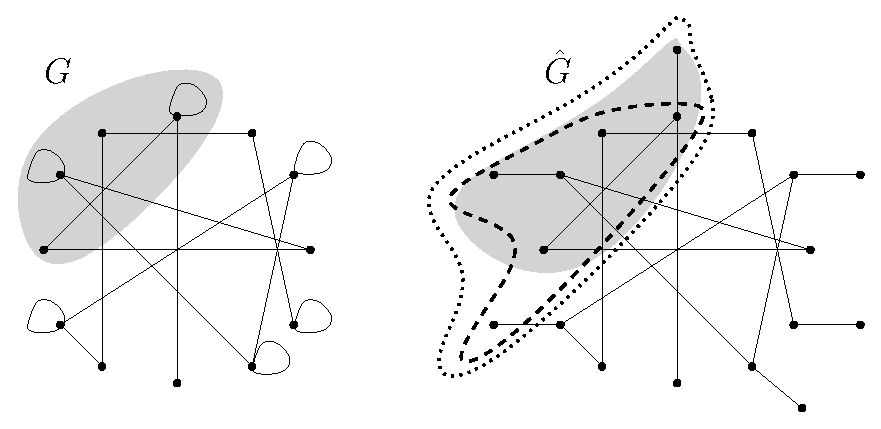
\includegraphics[scale=0.9]{cuts_selfloops.eps}
		\end{minipage}
		\caption{There is a straightforward correspondence between the shaded cuts in $G$ and $\hat{G}$, since they have same volume and same number of crossing edges. The dashed cut has missing self-loops and dangling self-loops (think of it as the cut $R$). The dotted cut adds the missing self-loops (think of it as the cut $Q$). The shaded cut in $\hat{G}$ removes the dangling self-loops (think of it as the cut $P$), and corresponds to the shaded cut in $G$ (think of it as the cut $X$).}
		\label{fig:selfloopscuts}
	\end{figure}

	\noindent
	We know from~\eqref{itdef:sparseapp} that
	\begin{equation*}
		\frac{\partial_{\hat{G}} R}{\vol_{\hat{G}} (R)} < \alpha \phi \, .
	\end{equation*}
	Consider the cut $Q=R \cup s(R \cap A)$, i.e. a version of $R$ where we have added the self-loops of all the vertices in $R$ that have one. Then $Q \subsetneq \hat{V}$, as otherwise $V \subseteq R$, which would imply that $R$ contains more than half the volume of $\vol_{\hat{G}}(\hat{V})$, contradicting~\eqref{itdef:smallsideapp}. Next, we remark that the volume of $Q$ cannot decrease compared to $R$, since we added vertices, i.e.
	\begin{equation}
		\label{eq:volrq}
		\vol_{\hat{G}}(Q) = \vol_{\hat{G}}(R) + \partial_{\hat{G}}(s(R \cap A) \setminus (R \cap B)) \ge \vol_{\hat{G}}(R)\, .
	\end{equation}
	At the same time, we do not increase the number of crossing edges since we move the self-loop edges inside the cut, so
	\begin{equation*}
		\frac{\partial_{\hat{G}} Q}{\vol_{\hat{G}}(Q)} = \frac{\partial_{\hat{G}} R - \partial_{\hat{G}}(s(R \cap A) \setminus (R \cap B))}{\vol_{\hat{G}}(R) + \partial_{\hat{G}}(s(R \cap A) \setminus (R \cap B))} \le \frac{\partial_{\hat{G}} R}{\vol_{\hat{G}} (R)} \, .
	\end{equation*}
	Thus, we have added self-loops to $R$ without increasing its sparsity nor decreasing its volume. Now we remove the dangling self-loops from $Q$, i.e. we remove the set $D=(Q \cap B) \setminus s(Q \cap A)$, and consider the cut $P=Q \setminus D$. We remark that $P \neq \emptyset$, as otherwise $R$ is solely made of vertices from~$s(A)$, which contradicts $\Phi_H(R) < \alpha \phi \le 1/10 < 1$. Since we removed an equal amount of mass from both the crossing edges and the volume, we get
	\begin{equation*}
		\frac{\partial_{\hat{G}} P}{\vol_{\hat{G}}(P)} \le \min\left\{\frac{\partial_{\hat{G}} P}{\vol_{\hat{G}}(P)}, 1\right\} \le \frac{\partial_{\hat{G}} P + \partial_{\hat{G}} D}{\vol_{\hat{G}}(P)+\partial_{\hat{G}} D}  = \frac{\partial_{\hat{G}} Q}{\vol_{\hat{G}} (Q)} \, .
	\end{equation*}
	Thus, removing the dangling self-loops does not increase sparsity. However we may have decreased the volume, which threatens the balancedness property of the cut. We then bound the decrease: because we proved before ${\partial_{\hat{G}} Q}/{\vol_{\hat{G}} (Q)} < \alpha \phi$, we know
	\begin{equation*}
		\partial_{\hat{G}} D < \frac{\alpha \phi}{1-\alpha\phi}\vol_{\hat{G}}(P) \, ,
	\end{equation*}
	so
	\begin{equation}
		\label{eq:volpq}
		\vol_{\hat{G}}(Q) = \vol_{\hat{G}}(P) + \partial_{\hat{G}} D < 2 \vol_{\hat{G}}(P) \, .
	\end{equation}
	Now one can see that $P$ is identical to $(R \cap V) \cup s(R \cap A)$, and $X$ as defined in Algorithm~\ref{alg:selfloop} equals $R \cap V$. Hence $\partial_G X = \partial_{\hat{G}} P$ and $\vol_G(X)=\vol_{\hat{G}}(P)$. Therefore,
	\begin{equation}
		\label{eq:smallratio}
		\frac{\partial_G X}{\vol_G (X)} < \alpha \phi \, .
	\end{equation}
	To handle the case where $X$ is the larger volume side of the cut, \cref{alg:selfloop} takes $X^*$ to be the side of $(X,V\setminus X)$ with smaller volume. We show that the volume of $V\setminus X$ is within a small constant factor of the volume of $X$. To do so, recall that $\Phi_{\hat{G}}(R)<\alpha \phi$, so
	\begin{equation*}
		\frac{\partial_{\hat{G}} Q + \partial_{\hat{G}}(s(R \cap A) \setminus (R \cap B))}{\vol_{\hat{G}}(Q) - \partial_{\hat{G}}(s(R \cap A) \setminus (R \cap B))} < \alpha \phi \,,
	\end{equation*}
	which implies
	\begin{equation*}
		\partial_{\hat{G}}(s(R \cap A) \setminus (R \cap B)) < \alpha \phi \vol_{\hat{G}}(Q) \, .
	\end{equation*}
	Hence, by property~\eqref{itdef:smallsideapp} of $R$, we have
	\begin{equation*}
		\vol_G(X) \le \vol_{\hat{G}}(Q) < \frac{1}{1-\alpha\phi}\vol_{\hat{G}}(R) \le \frac{1}{2} \cdot  \frac{1}{1-\alpha\phi} \vol_{\hat{G}}(\hat{V}) = \frac{1}{2} \cdot  \frac{1}{1-\alpha\phi}\vol_G(V) \, .
	\end{equation*}
	Therefore, we have that $X^* = \argmin\{\vol_G(X), \vol_G(V\setminus X)\}$ satisfies
	\begin{equation}
			\label{eq:nearlysamevol}
		(1-2\alpha\phi)\vol_G(X) \le \vol_G(X^*) \le \vol_G(V\setminus X^*) \, ,
	\end{equation}
	and
	\begin{equation}
		\label{eq:largevol}
		\vol_{\hat{G}}(R) < \frac{2}{1-2\alpha \phi}\vol_G(X^*) \, ,
	\end{equation}
by~\eqref{eq:volrq},~\eqref{eq:volpq}. We now conclude by verifying properties~\eqref{itdef:sparseapp2},~\eqref{itdef:smallsideapp2},~\eqref{itdef:balapp2},~\eqref{itdef:goodestimapp2}.

\begin{itemize}
	\item \textit{Property~\eqref{itdef:sparseapp2}.} From~\eqref{eq:smallratio} and~\eqref{eq:nearlysamevol}, we get $\Phi_G(X^*) < 	\alpha\phi /({1-2\alpha \phi}) \le 2 \alpha \phi$.
	\item \textit{Property~\eqref{itdef:smallsideapp2}.} This property follows by definition of $X^*$ in \cref{alg:selfloop}.
	\item \textit{Property~\eqref{itdef:balapp2}.} Consider any cut $\emptyset \neq T \subsetneq V$ such that $\Phi_G(T) < \phi$ and $\vol_G(T) \le \vol_G(V \setminus T)$. Then we know that
	\begin{equation*}
		\Phi_G(T) = \Phi_{\hat{G}}(T \cup s(T \cap A)) < \phi \, ,
	\end{equation*}
	and
	\begin{equation*}
		\vol_{\hat{G}}(T \cup s(T \cap A)) = \vol_G(T) \le \vol_G(V \setminus T) = \vol_{\hat{G}}(\hat{V} \setminus (T \cup s(T \cap A))\, ,
	\end{equation*}
	as well as
	\begin{equation*}
		\vol_G(T) = \vol_{\hat{G}}(T \cup s(T \cap A)) \le \lambda \cdot \vol_{\hat{G}}(R) < \frac{2\lambda}{1-2\alpha \phi}\vol_G(X^*) \le 4\lambda \vol_G(X^*)\, ,
	\end{equation*}
	by an application of~\eqref{itdef:balapp} to the cut $T \cup s(T \cap A)$ and~\eqref{eq:largevol}.
	\item \textit{Property~\eqref{itdef:goodestimapp2}.} Follows directly by definition of $\omega$ in \cref{alg:selfloop}.
\end{itemize}
\end{proof}
\noindent
Using \cref{lem:selfloopfree}, we now conclude a proof of \cref{th:fastbalsparse}. To do so, we run two different algorithms, depending on how large $p$ and $q$ are.

\paragraph{The large case.}
An algorithm was recently given that, for $p$-vertex $q$-edge input graphs with edge weights bounded by $\poly(p)$ produces a $(O(\phi \log^3 p), \phi)$-ED\footnote{In this case, the definition of ED uses the weight of edges across cuts, and weighted volumes, including self-loops.} with probability $1-1/\poly(p)$ in $(p+q)\cdot \pylog(p)$ time, for any $\phi \in (0,1)$~\cite{liexpdec}. One can then use this ED algorithm to efficiently compute an approximate balanced $\psi$-sparse cut for all $\psi \in (0,1)$: as it was observed in~\cite{offlineexpdec}, given access to a graph and its $(O(\psi \log^3p), \psi)$-ED, one can easily obtain a $(\psi,c' \cdot \log^3 p, C',0)$-BSCW for some constants $c',C'\ge 1$. This gives a $(c' \cdot \log^3 p, C')$-BSCA that runs in $(p+q)\cdot \pylog(p)$ time for all input sparsity parameters~$\psi \in (0,1)$.

Whenever $p \ge n^{1/c_{\text{time}}}$, for a constant $c_{\text{time}} \ge 1$ to be determined later, we then apply the algorithm of \cite{offlineexpdec,liexpdec} together with \cref{lem:selfloopfree} setting $\alpha=c' \log^3 n$ and $\lambda = C'$ (where $c',C'\ge 1$ are the constants one gets from the self-loop free BSCA of~\cite{offlineexpdec,liexpdec}). Then, we get a $(c_{\sw} \log^3 n,C_{\sw})$-BSCA where $c_{\sw}=2c'$ and $C_{\sw} = 4C'$, provided that \smash{$\phi \le \frac{1}{10\alpha}$}. Using $\phi = \psi$ and since we impose \smash{$\psi \le  \frac{1}{10 c_{\sw} \log^3 n}$}, we get \smash{$\phi \le \frac{1}{10\alpha}$}.

Using our assumption on $p,q,W$, the space and random bit complexity trivially follow from the bound on the running time, which is in turn at most $\poly(n)$. The success probability is $1-1/\poly(p)$, which gives the claimed success probability of $1-1/\poly(n)$.


\paragraph{The small case.}
When $p < n^{1/c_{\text{time}}}$, we use an algorithm running in $T(p,q,W)$ time. The algorithm consists in using an algorithm that $(c'' \log p)$-approximates the sparsity of the input graph (such as the deterministic polynomial time algorithm of \cite{leightonrao,llr}, which allows to have weighted self-loops by incorporating them in the demand graph) as follows (which is essentially the idea of \cite{offlineexpdec}): maintain a cut $R$ initially empty and repeatedly compute the approximate sparsest cut $S$ of $G[V\setminus R]^1$; if $S$ has sparsity at least $2\psi c'' \log p$ then terminate, else update $R$ to be $R \cup S$; if  $R$ accounts for at least a $1/5$ fraction of the total volume of $G$ then terminate, else repeat.

First note that this algorithm terminates (e.g. when $V \setminus R$ is a single vertex). Also observe that if $R = \emptyset$ then we can conclude that $G$ is a $2\psi$-expander. Otherwise, $R$ has always sparsity at most $4\psi c'' \log p$ in $G$ and one of $R,V\setminus R$ hs volume at most half of the total. Moreover, if the smaller of $R,V\setminus R$ accounts for at least a $1/5$ fraction of the total volume of $G$ then every $\psi$-sparse cut with volume at most half the total is within a $5/3$ fraction of the volume of the smaller of $R,V\setminus R$. Finally, if $R$ accounts for less than a $1/5$ fraction of the total volume of $G$, then $G[V\setminus R]^1$ is a $2\psi$-expander; consider a cut $T$ with sparsity at most $\psi$ and volume at most half the total; then if $T$ had more than half its volume in $V \setminus R$, the weight of edges crossing the cut $T$ in $G$ would be more than a $\psi$ fraction of the volume of $T$, a contradiction; hence, $T$ is within a factor of $2$ of the volume of $R$. This gives a $(c'' \log n,2)$-BSCA.

We pick $c_{\text{time}}$ so that $T(p,q,W)$ is at most \smash{$\otil(n/b^2)\cdot \log^{O(\frac{\log n}{\log 1/b})}n$}, thus giving the claimed bound on the space and random bit complexity. In our case, $T(p,q,W)=\poly(p,q,\log W)$ (which can be achieved by solving the linear programming relaxation of \cite{leightonrao} with the ellipsoid method and rounding it deterministically with the algorithm of \cite{llr}) and recall that $W=\poly(n)$, so there exists a constant $c_{\text{time}} \ge 1$ such that $T(p,q,W)$ is at most \smash{$n/b^2 \cdot \log^{O(\frac{\log n}{\log 1/b})}n$}. The running time also follows, and the success probability is $1$.
\\~\\
 \cref{th:fastbalsparse} is concluded by combining the large and small case.

\end{proof}

\subsection{Expansion and regularity of random graphs}
\label{apndx:randomgraphs}
\erdos*
\begin{proof}
	Let $H=(U,F)$ be a sample from $\er(N,p)$, so that $|U|= N$. Also let $L=D-A$ be the Laplacian matrix of $H$, where $D$ denotes its degree diagonal matrix and $A$ denotes its adjacency matrix. We use the following matrix Bernstein concentration bound on $L$ to lower bound its second eigenvalue, and then lower bound the expansion of $H$ using Cheeger's inequality.
	\begin{theorem}[Theorem 1.6.2 in~\cite{matcon}]
		\label{th:bern} Let $S_1,\dots, S_\kappa \in \mathbb{R}^{N \times N}$ be independent symmetric random matrices such that $\ex[S_\iota]=0$ and $\nm{S_\iota} \le \lambda$ for every $\iota \in [\kappa]$, and let $S = \sum_{\iota=1}^{\kappa} S_\iota$. Then, for all~$\theta \ge 0$
		\begin{equation*}
			\Pr[\nm{S} \ge \theta] \le 2N \cdot \exp\left(-\frac{\theta^2/2}{\nm{ \sum_{\iota=1}^{\kappa} \ex[S_\iota^2]}+\lambda\theta/3}\right) \, .
		\end{equation*}
	\end{theorem}
	\noindent
	We start by rewriting $L$ so that we can apply the above result. For each $e=\{u,v\} \in \binom{V}{2}$ let $z_e \sim \ber(p)$ be an independent Bernoulli random variable with bias $p$, and also let $L_e $ be the Laplacian matrix of the graph $(U,\{e\})$, i.e. $(L_e)_{ab} = 1$ if $a=b=u$ or $a=b=v$, $(L_e)_{ab} = -1$ if $\{a,b\}=e$, and $(L_e)_{ab}=0$ otherwise. Define $S_e = z_e L_e - \ex[z_eL_e]$ and \smash{$S = \sum_{e \in \binom{V}{2}} S_e$}. One can now note that
	\begin{equation*}
		\ex[S_e]=0 \quad \text{and} \quad \nm{S_e} \le \max\left\{\nm{(1-p)L_e},\nm{-pL_e}\right\} \le 2\quad \text{for all $e\in \binom{V}{2}$.}
	\end{equation*}
	Letting $J$ be the all-ones $N \times N$ matrix we  also have
	\begin{equation*}
		S = \sum_{e \in \binom{V}{2}} z_e L_e - \sum_{e \in \binom{V}{2}} \ex[z_eL_e] = L- p \cdot (N \cdot I-J)\, .
	\end{equation*}
	Hence, \cref{th:bern} with $\lambda=2$ gives
	\begin{equation}
		\label{bern:appl}
		\Pr[\nm{L-p \cdot (N \cdot I-J)} \ge \theta] \le 2N \cdot \exp\left(-\frac{\theta^2/2}{\nm{ \sum_{e \in \binom{V}{2}} \ex[(z_e L_e - \ex[z_eL_e])^2]}+2\theta/3}\right) \,.
	\end{equation}
	Now we observe that the first term in the denominator can be rewritten as
	\begin{align*}
		\nm{ \sum_{e \in \binom{V}{2}} \ex\left[(z_e L_e - \ex[z_eL_e])^2\right]} & = \nm{ \sum_{e \in \binom{V}{2}} 2L_e\ex\left[(z_e-z_e\cdot p+p^2)\right]} \\
		& = \nm{ \sum_{e \in \binom{V}{2}} 2pL_e} \\
		& = 2p \nm{N \cdot I-J} \\
		& = 2pN	\, ,
	\end{align*}
	where the last equality holds because $K \coloneqq N \cdot I-J$ is the Laplacian matrix of the complete graph on $N$ vertices. If we now set $\theta = pN/10$ in~\eqref{bern:appl}, we get
	\begin{equation}
		\label{eq:specapprox}
		\Pr\left[\nm{L-p \cdot K} \ge \frac{1}{10}pN\right] \le  2N \cdot \exp\left(-\frac{pN}{600}\right) \, .
	\end{equation}
	Now, in order to use a Cheeger type of inequality, it is convenient to view $H$ as a regular graph, so that its normalized Laplacian matrix is simply a scalar multiple of $L$. If we denote with $\deg(u)$ the degree of $u \in U$ in $H$, we get by a Chernoff bound that
	\begin{equation}
		\label{eq:degrees}
		\Pr\left[\text{$\exists u \in U$, } \left|\deg(u) - p\cdot (N-1)\right| > \frac{1}{14}p \cdot (N-1)\right] \le 2N \cdot \exp\left(-\frac{p\cdot (N-1)}{600}\right) \,.
	\end{equation}
	From~\eqref{eq:specapprox} and~\eqref{eq:degrees}, we then have
	\begin{equation}
		\label{eq:sectolast}
			\Pr\left[\left(\nm{L-p K} \ge \frac{1}{10}pN\right)\text{ or } \left(\exists u \in U : \left|\deg_H(u)-\bar{d}\right|>\frac{1}{14} \bar{d}\right)\right] \le 4N \cdot \exp\left(-\frac{pN}{600}\right) \, .
	\end{equation}
	We conclude by showing that if the event in the above probability does not occur, then the event argument of the probability in the statement of \cref{prop:er} does not occur either. To see this, let $\lambda_2$ be the second smallest eigenvalue of $1/\bar{d}  \cdot L$, and $\mu_2$ be the second smallest eigenvalue of $1/(N-1) \cdot K$. Hence, $\nm{L-p K} < \frac{1}{10}pN$ implies $\lambda_2 \ge \mu_2-1/9$ by Weyl's inequality. Moreover, we know that $\mu_2 = N/(N-1)$, so $\lambda_2 \ge 9/10$. Finally, let $\emptyset \neq S \subsetneq U$ be a cut with $\vol(S) \le \vol(U\setminus S)$ such that $\Phi_H(S) = \Phi_H$. Assuming $\left|\deg_H(u)-\bar{d}\right|\le \frac{1}{14} \bar{d}$ for all $u \in U$, we have that $\vol(S) \in [(1-1/14)\bar{d} |S|, (1+1/14)\bar{d} |S|]$. Let $\vt{y} \in \mathbb{R}^U$ be defined as $y_u = 1/|S|$ if $u \in S$ and $y_u=-1/|U \setminus S|$ otherwise. By Courant-Fischer we then have
	\begin{align}
		\label{eq:courfisch}
		\lambda_2 = \min_{\substack{\vt{x} \in \mathbb{R}^U\setminus \{\vt{0}\}:\\ \langle \vt{x}, \ind \rangle= 0}} \, \frac{1}{\bar{d}} \cdot \frac{\vt{x}^\top L\vt{x}}{ \vt{x}^\top \vt{x}} \le \frac{1}{\bar{d}} \cdot  \frac{\vt{y}^\top L\vt{y}}{\vt{y}^\top \vt{y}}  = \frac{\uncut{S}{U}}{\bar{d}|S|} \cdot \frac{|U|}{|U\setminus S|}  \le \left(1+\frac{1}{14}\right)\Phi_H \cdot \frac{|U|}{|U\setminus S|} \, .
	\end{align}
	Again assuming $\left|\deg_H(u)-\bar{d}\right|\le \frac{1}{14} \bar{d}$ for all $u \in U$, one can check that $\vol(S) \le \vol(U\setminus S)$ implies $|U\setminus S| \ge 6/7 \cdot |S|$. Thus,~\eqref{eq:courfisch} gives
	\begin{equation*}
		\lambda_2 \le \left(1+\frac{1}{14}\right)\cdot \left(1+\frac{7}{6}\right) \Phi_H \le \frac{27}{10} \Phi_H \, ,
	\end{equation*}
	so $\Phi_H \ge 1/3$.
\end{proof}

\subsection{A useful inequality}
\label{apndx:ineq}
\math*
\begin{proof}
	Write $x=y\cdot \e^{\rho-1}$ for some $\rho \le 1$. Then $(y/x)^x \le \e^{y/\e}$ if and only if $(1-\rho)e^{\rho-1} \le 1/\e$. Define $f(\rho)=(1-\rho)\e^{\rho}$. We prove the claim by showing that $f(\rho) \le 1$ for all $ \rho \in (-\infty, 1]$.
	
	We begin by noting that $f$ is continuous over $(-\infty, 1]$. Then, we take the derivative of $f$, and we get $f'(\rho)=-\rho \e^\rho$. We observe that $f'(\rho) > 0$ for $\rho <0$, and $f'(\rho) > 0$ for $\rho >0$. We further observe that $f(0) = 1$, $f(1)=0$, and $\lim_{\rho \rightarrow -\infty} f(\rho) = 0$. Hence, $f(\rho)$ is upper-bounded by $1$ for all~$\rho \in (-\infty, 1]$.
\end{proof}
